\documentclass[12pt]{article}

\usepackage{amsmath, amssymb}
\usepackage{graphicx}
\usepackage{natbib}
\usepackage{setspace}
\usepackage{hyperref}
\usepackage{geometry}
\usepackage{indentfirst}
\usepackage{tikz}
\usetikzlibrary{positioning, arrows}

\geometry{margin=1.1in}

\begin{document}
\begin{titlepage}
    \centering
    \vspace*{2cm}

    {\Huge\bfseries Graph-theoretic Models and Algorithms for Imprecise Probabilities	 \par}
    \vspace{0.5cm}
    {\LARGE Dempster--Shafer Theory and Credal Networks\par}
    \vspace{2.5cm}

    {\Large David Castrejon\par} % Replace with your name
    \vspace{0.5cm}
    {\large Johns Hopkins University\par} % Optional affiliation
    \vfill

    \vspace{1cm}

\end{titlepage}

\section*{Overview}

Reasoning under uncertainty remains a key challenge in AI and decision-making, especially in situations where the underlying probabilities are not fully known. Traditional probability theory requires knowledge of all relevant distributions, but in practice, data is often incomplete, evidence may conflict, and precise probabilities cannot be reliably determined. Such limitations motivate the development of models that extend classical probabilistic frameworks to handle imprecision, uncertainty, and partial knowledge. Among these, Dempster–Shafer (DS) theory offers a well-established mechanism for representing uncertainty through belief functions \cite{shafer1976}, which generalize probabilities by assigning masses to sets of outcomes rather than individual events. This approach allows for the combination of evidence from multiple sources using Dempster’s rule of combination, providing a flexible method for reasoning under conditions of partial or conflicting information. Complementing DS theory, credal networks \cite{cozman2005} , as introduced by Cozman, generalize Bayesian networks by allowing conditional probabilities to be specified as sets or intervals rather than single point estimates. These frameworks together illustrate a collection of approaches for reasoning under uncertainty.

\section*{Problem Statement}

The core problem motivating these frameworks arises from the observation that Bayesian networks require precise conditional probabilities for all variables \cite{koller2009}. However, many domains involve incomplete or ambiguous knowledge, making precise specification either impractical or impossible. This motivates the central question of our study: what methods allow us to represent and propagate uncertainty when probabilities are not precisely specified? Addressing this question is critical for enabling AI systems to perform realistic reasoning under uncertainty. This applies to domains such as sensor fusion, risk assessment, and decision support systems, where evidence may be incomplete or contradictory. Prior work provides partial answers. Dempster–Shafer theory, first developed by Dempster in 1967 \cite{dempster1967} and formalized by Shafer in 1976 \cite{shafer1976}, introduces belief functions as a way to assign support to both individual hypotheses and sets of hypotheses. Cozman’s graphical models for imprecise probabilities extend this idea by defining credal networks, where conditional probabilities are represented as convex sets of distributions  \cite{cozman2005}, allowing imprecision to be encoded systematically while retaining the conditional independence structure of Bayesian networks. Together, these approaches provide a framework for reasoning under uncertainty that bridges the gap between fully specified probabilistic models and complete ignorance.

\section*{Study Approach}

\subsection*{Findings and Contributions of Cozman}

In his 2005 paper, Cozman lays out both the theoretical foundations and practical considerations for credal networks, which perform inference over sets of probabilities instead of single-point distributions \cite{cozman2005}. The paper positions credal networks as a natural generalization of Bayesian networks in which each conditional probability table is replaced by a convex set of admissible conditional distributions. This shift from point-valued to set-valued probabilities enables the representation of epistemic uncertainty, incompleteness, and expert disagreement in a way that Bayesian networks inherently cannot. \newline

The paper introduces several ideas that serve as part of the foundation of
credal network theory. First, Cozman defines the local credal set
$K(X_i \mid \mathrm{pa}(X_i))$ for each node, representing all conditional
probability distributions consistent with available knowledge. Second, the paper
distinguishes between two independence concepts: strong
independence, which requires independence to hold for every distribution in the
credal set, and epistemic independence, which encodes a weaker form of
independence based on uncertainty rather than factorization. These notions lead
to the definition of the strong extension of a credal network, the
largest joint credal set consistent with all local constraints and the chosen
independence assumption. Cozman shows that strong extensions possess a
factorization property closely paralleling Bayesian networks, making them the
most analytically tractable of the possible credal constructions. \newline

Cozman’s work also highlights the computational difficulties involved in credal inference. He shows that calculating exact marginal bounds in general credal networks is NP-hard, even for relatively simple network structures. For multiply connected networks, exact inference is often
intractable due to the need to evaluate all extreme points of the strong
extension, whose number may grow exponentially with the number of variables. The
paper shows that this complexity persists even when all local credal sets are
specified by only two extreme points per conditional distribution \cite{cozman2000}. These results
portray the need for approximation techniques and justify the importance of
studying simplified methods such as the exhaustive extreme-point enumeration
used in this project. \newline

Despite these complexity barriers, Cozman also identifies classes of networks
in which tractable inference is possible. For instance, when the credal network
is a polytree and independence is interpreted in the strong sense, exact
computation of lower and upper probabilities can be performed by variants of
belief propagation applied to extreme points. The paper further discusses
approximate inference methods such as Tessem’s A/R and A/R+ algorithms, which
propagate outer approximations of credal sets using interval-valued messages,
offering a trade-off between computational efficiency and precision. \newline

The findings by Cozman provide a theoretical reference point for the
present study. My implementation of a credal network follows the simplest exact method suggested by Cozman. Explicit enumeration of extreme points of local credal sets to form the strong extension followed by computation of marginal bounds across these distributions \cite{cozman2005}. While this approach does not scale to large or multiply connected
networks, it is consistent with the foundational principles articulated by
Cozman and allows us to empirically confirm the behavior of credal networks on
small-scale examples. By comparing these results with those of Dempster–Shafer
theory, we directly engage with Cozman’s central finding, which is that imprecise probabilistic formalisms can generalize classical graphical models while capturing degrees of ignorance that traditional Bayesian networks cannot represent. \newline


Imprecise probabilities extend classical probability theory by working with sets or ranges of possible distributions. This approach allows models to account for partial knowledge, conflicting evidence, and uncertainty in a mathematically consistent manner. In DS theory, belief functions are defined via mass functions \(m: 2^\Theta \rightarrow [0,1]\), where \(\Theta\) is the frame of discernment, satisfying

\begin{equation}
\sum_{A \subseteq \Theta} m(A) = 1, \quad m(\emptyset) = 0.
\end{equation}

The belief function \(\text{Bel}(A)\) and plausibility function \(\text{Pl}(A)\) are then defined as

\begin{equation}
\text{Bel}(A) = \sum_{B \subseteq A} m(B)
\end{equation}

\begin{equation}
\text{Pl}(A) = \sum_{B \cap A \neq \emptyset} m(B)
\end{equation}

providing lower and upper bounds on the probability of the proposition \(A\). Dempster’s rule of combination, which merges two independent sources of evidence \(m_1\) and \(m_2\), is given by

\begin{equation}
(m_1 \oplus m_2)(C) = \frac{1}{1-K} \sum_{A \cap B = C} m_1(A)m_2(B), \quad K = \sum_{A \cap B = \emptyset} m_1(A)m_2(B),
\end{equation}

where \(K\) quantifies the conflict between sources. Marginalization over a variable \(X\) is expressed as

\begin{equation}
m_Y(B) = \sum_{A: A|_Y = B} m_X(A),
\end{equation}

allowing local computation on graphs as formalized by Shenoy and Shafer. Credal networks extend these ideas by replacing point-valued conditional probabilities \(P(X_i | \text{Pa}(X_i))\) with sets of distributions \(\mathcal{K}(X_i | \text{Pa}(X_i))\), where each credal set represents all distributions consistent with constraints \cite{cozman2005}:

\begin{equation}
\mathcal{K}(X_i | \text{Pa}(X_i)) = \{ P(X_i | \text{Pa}(X_i)) \, | \, l_{ij} \leq P(X_i=x_j|\text{Pa}(X_i)) \leq u_{ij} \},
\end{equation}

maintaining the conditional independence relationships central to Bayesian network reasoning. \newline

To illustrate the practical behavior of Dempster--Shafer theory and credal networks under partially specified knowledge, I have implemented small-scale diagnostic networks comprising four variables: Flu, Cold, Fever, and Cough. For DS theory, mass functions were assigned to each node based on expert knowledge and observed frequencies, allowing mass to be placed on singletons as well as composite sets to reflect partial or ambiguous evidence. Belief and plausibility intervals were computed using the Shenoy--Shafer local computation rules, systematically combining and marginalizing evidence from parent nodes. For credal networks, conditional probabilities were specified as intervals, representing partial knowledge or epistemic uncertainty. Marginal bounds were computed using extreme-point analysis, iterating over all feasible combinations of parent extreme points to provide mathematically rigorous lower and upper probabilities for each node \cite{cozman2000}.

\section*{Results}

\subsection*{Dempster--Shafer Theory}

The DS network produced the following marginal belief and plausibility intervals:

\begin{table}[h!]
\centering
\begin{tabular}{lcc}
\hline
\textbf{Node} & \textbf{Belief (Present)} & \textbf{Plausibility (Present)} \\
\hline
Flu   & 0.036 & 0.048 \\
Cold  & 0.111 & 0.125 \\
Fever & 0.025 & 0.029 \\
Cough & 0.067 & 0.078 \\
\hline
\end{tabular}
\caption{Marginal belief and plausibility intervals obtained from the DS network.}
\end{table}

\begin{figure}[h!]
\centering
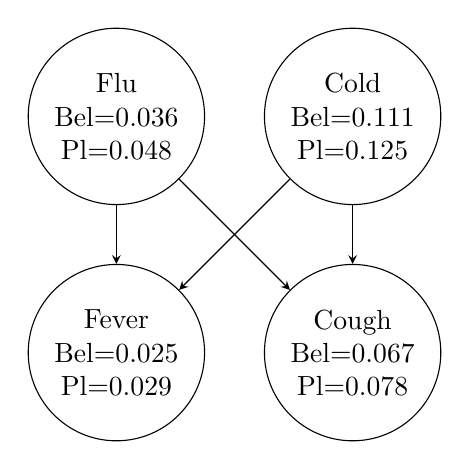
\begin{tikzpicture}[>=stealth, node distance=3cm, every node/.style={draw, circle, align=center}]
    \node (flu) {Flu\\Bel=0.036\\Pl=0.048};
    \node (cold) [right of=flu] {Cold\\Bel=0.111\\Pl=0.125};
    \node (fever) [below of=flu] {Fever\\Bel=0.025\\Pl=0.029};
    \node (cough) [below of=cold] {Cough\\Bel=0.067\\Pl=0.078};

    \draw[->] (flu) -- (fever);
    \draw[->] (cold) -- (fever);
    \draw[->] (flu) -- (cough);
    \draw[->] (cold) -- (cough);
\end{tikzpicture}
\caption{Graphical representation of the DS network with belief and plausibility intervals.}
\end{figure}


Root nodes Flu and Cold had direct mass assignments, yielding narrow and interpretable intervals. Child nodes Fever and Cough, influenced by propagated evidence, exhibit slightly larger but still narrow intervals, reflecting modest residual uncertainty. \newline


\subsection*{Credal Network}

The credal network analysis yielded the following marginal probability bounds:

\begin{table}[h!]
\centering
\begin{tabular}{lcc}
\hline
\textbf{Node} & \textbf{Lower Bound} & \textbf{Upper Bound} \\
\hline
Flu   & 0.05   & 0.10   \\
Cold  & 0.10   & 0.20   \\
Fever & 0.00   & 0.1615 \\
Cough & 0.00   & 0.1330 \\
\hline
\end{tabular}
\caption{Marginal probability bounds obtained from the credal network using extreme-point analysis. \cite{cozman2000}}
\end{table}

\begin{figure}[h!]
\centering
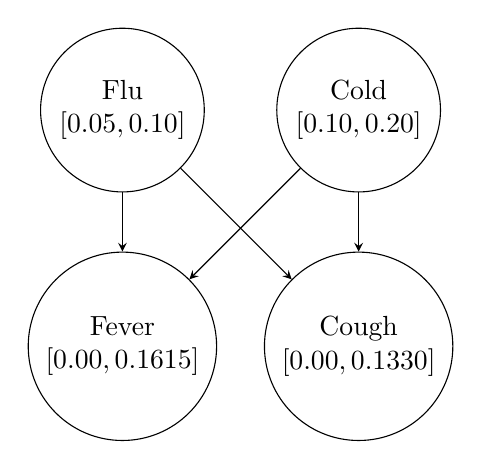
\begin{tikzpicture}[>=stealth, node distance=3cm, every node/.style={draw, circle, align=center}]
    \node (flu) {Flu\\$[0.05,0.10]$};
    \node (cold) [right of=flu] {Cold\\$[0.10,0.20]$};
    \node (fever) [below of=flu] {Fever\\$[0.00,0.1615]$};
    \node (cough) [below of=cold] {Cough\\$[0.00,0.1330]$};

    \draw[->] (flu) -- (fever);
    \draw[->] (cold) -- (fever);
    \draw[->] (flu) -- (cough);
    \draw[->] (cold) -- (cough);
\end{tikzpicture}
\caption{Graphical representation of the credal network with lower and upper probability bounds.}
\end{figure}

Root node bounds correspond exactly to the input intervals, while child nodes exhibit bounds determined by all feasible combinations of parent extreme points. Notably, Fever and Cough have lower bounds at zero, reflecting that the absence of parent conditions is consistent with the model. This illustrates the credal network’s capability to provide rigorous, guaranteed bounds under imprecise probability specifications, offering mathematically robust reasoning about uncertainty.

\subsection*{Comparative Analysis}

It is important to note that the Dempster–Shafer model used in this paper does not employ interval-valued mass assignments or sets of belief functions. The basic probability assignments in our DS network are point-valued (e.g., $m(\text{Flu}) = 0.1$, $m(\text{NoFlu}) = 0.8$, $m(\{\text{Flu, NoFlu}\}) = 0.1$). Unlike credal networks, which represent imprecision directly in the network parameters through probability intervals or sets of conditional distributions, the DS model concentrates uncertainty in the focal sets themselves. Nonetheless, DS inference naturally produces interval-valued results through the belief and plausibility measures. These measures define lower and upper bounds on the probability of each event—e.g., $P(\text{Fever}) \in [Bel(\text{Fever}), Pl(\text{Fever})]$. Thus, although the two frameworks both yield interval-valued uncertainty at the inference level, the source and interpretation of these intervals differ substantially. Credal networks encode imprecision structurally in the model parameters, whereas Dempster–Shafer 
theory expresses imprecision through the belief–plausibility calculus applied after 
evidence combination. \newline

Comparing the results of the DS network and the credal network provides important insights into how these frameworks handle uncertainty. In DS theory, belief and plausibility intervals explicitly incorporate both partial support and conflict among evidence sources, whereas credal networks provide guaranteed probability bounds that encompass all distributions consistent with the specified intervals \cite{cozman2005}. The magnitude and symmetry of the intervals differ between the frameworks. In this network, DS intervals for child nodes remain narrow due to low residual ignorance, reflecting minimal conflict in the available evidence. Meanwhile credal network bounds are mathematically tight with lower bounds that can reach zero, reflecting the full range of uncertainty. Propagation behavior also varies. DS theory can sometimes produce counterintuitive interval widths due to the combination of conflicting parent evidence \cite{shafer1976}, while credal networks systematically evaluate all feasible configurations of parent nodes, yielding more rigorous marginal bounds. These differences have interpretational consequences. DS theory is particularly useful for analyzing evidence aggregation and conflict resolution, providing intuitive measures of belief and plausibility. Whereas credal networks are better suited for formal reasoning under partial knowledge, offering precise bounds that support worst-case and best-case decision-making. Computationally, both frameworks face challenges. For example, DS propagation becomes expensive as the frame of discernment grows. Especially in multiply connected networks, while credal networks encounter combinatorial complexity when enumerating extreme points \cite{cozman2000}. However, credal networks can leverage convex optimization techniques to scale more effectively than DS theory in certain contexts \cite{koller2009}. \newline

These results suggest that DS theory focuses on directly capturing conflict among evidence and the residual uncertainty it produces, offering measures that are both interpretable and operational. Credal networks take a more formal approach, encoding conditional probabilities as convex sets and producing bounds that rigorously account for uncertainty, which is useful for decision-making \cite{cozman2005}. In combination, they illustrate a continuum of reasoning under uncertainty, from belief-function propagation to interval-based probabilistic reasoning, highlighting complementary strengths in the representation, propagation, and interpretation of uncertainty. \newline

While both Dempster–Shafer theory and credal networks provide principled methods for reasoning under uncertainty, they differ significantly in computational demands. In DS theory, the combination and marginalization of belief functions can become computationally expensive because the number of subsets in the frame of discernment grows exponentially with the number of variables. Multiply connected networks exacerbate this problem, as evidence must be propagated across multiple paths, leading to repeated calculations of conflicting mass and normalization steps. As a result, exact inference in large DS networks often becomes infeasible, necessitating approximate methods or heuristic simplifications. Credal networks, while more flexible in representing imprecise probabilities, also face computational challenges. Computing exact lower and upper bounds for marginal probabilities requires optimization over all extreme points of the credal sets, a process that can grow exponentially with the number of variables and the size of the sets \cite{cozman2000}. However, credal networks can leverage techniques from linear and convex programming, and in some cases, local propagation algorithms can exploit network sparsity to reduce computational load. Both frameworks therefore illustrate a fundamental trade-off in reasoning under uncertainty. DS theory emphasizes interpretability and conflict management whereas credal networks provide broader generality and mathematically guaranteed bounds at the cost of increased computational complexity. Understanding these limitations is essential for selecting the appropriate framework based on the size, connectivity, and nature of the domain under investigation. \newline

\section*{Conclusion}

Graphical models of imprecise probabilities offer a spectrum of methods for reasoning under uncertainty, trading off computational demands with flexibility and interpretability. DS theory supports belief-function propagation that is both practical and interpretable, making it particularly useful in situations where data is incomplete or conflicting. Credal networks generalize this approach through convex sets of conditional probabilities, enabling mathematically rigorous inference over partially specified models \cite{cozman2005}. Both frameworks demonstrate predictable and coherent behavior. DS theory produces belief and plausibility intervals reflecting evidence agreement and conflict, while credal networks yield bounds on probabilities that capture partial knowledge. Together, they illustrate complementary strengths in AI reasoning under uncertainty \cite{koller2009}, providing robust decision-making tools for real-world environments.

\newpage
\bibliographystyle{plainnat}
\begin{thebibliography}{}

\bibitem[Koller(2009)]{koller2009}
Daphne Koller and Nir Friedman.
\newblock Probabilistic Graphical Models: Principles and Techniques.
\newblock MIT Press, Cambridge, 2009.

\bibitem[Cozman(2000)]{cozman2000}
Fabio Gagliardi Cozman.
\newblock Credal networks.
\newblock \emph{Artificial Intelligence}, 120(2):199--233, 2000.

\bibitem[Cozman(2005)]{cozman2005}
Fabio Gagliardi Cozman.
\newblock Graphical models for imprecise probabilities.
\newblock \emph{International Journal of Approximate Reasoning}, 39(2--3):167--184, 2005.

\bibitem[Dempster(1967)]{dempster1967}
A.~P. Dempster.
\newblock Upper and lower probabilities induced by a multivalued mapping.
\newblock \emph{Annals of Mathematical Statistics}, 38(2):325--339, 1967.

\bibitem[Shafer(1976)]{shafer1976}
Glenn Shafer.
\newblock \emph{A Mathematical Theory of Evidence}.
\newblock Princeton University Press, 1976.

\end{thebibliography}

\section*{Appendix A: Code Availability}
All Python scripts used to construct the Dempster--Shafer belief network, the credal network, and the associated figures are included as supplementary materials. These files reproduce the results by printing them to standard output.

\section*{Appendix B: Reproducibility Notes}

All experiments reported in this paper were conducted using Python~3.12.12 on an Apple 
M1 MacBook Pro. The full source code used to implement both the Dempster--Shafer 
model and the credal network is included with this submission. The files are:

\begin{itemize}
    \item \texttt{dempster\_shafer.py} --- Computes mass functions, combined evidence, 
    and belief/plausibility values for the DS network using the Shenoy--Shafer 
    propagation approach.
    \item \texttt{credal.py} --- Implements interval-valued conditional probabilities 
    and computes marginal lower and upper bounds using extreme-point enumeration.
\end{itemize}

\subsection*{Execution Instructions}

To reproduce the results:

\begin{enumerate}
    \item Open a terminal (or command prompt) on your computer.
    \item Navigate to the folder containing the source code using the \texttt{cd} command. For example:
    \begin{verbatim}
    cd /path/to/your/code/folder
    \end{verbatim}
    \item Run the Dempster--Shafer script:
    \begin{verbatim}
    python3 dempster_shafer.py
    \end{verbatim}
    This will print all mass functions, combined evidence, and belief/plausibility values for the example medical diagnosis network.

    \item Run the Credal network script:
    \begin{verbatim}
    python3 credal.py
    \end{verbatim}
    This will compute and display marginal lower and upper probability bounds for each node in the network using the extreme-point enumeration method.

    \item No additional packages are required; both scripts rely solely on the Python standard library.
\end{enumerate}

Following these steps will reproduce all results presented in the Results section, including printed intermediate computations, propagated beliefs, and final marginal bounds.

\end{document}

